\section{Literature Review}

In this introductory chapter, we first present a brief historical overview of the evolution of Employee Stock Options (ESOs), the reasons behind their adoption, and the main issues related to their valuation and incentive alignment. We then focus on the reload feature, which allows the holder to receive a new option when exercising the original one, with a special focus on the more recent Dynamic Employee Stock Options (DESOs), which allow the holder to receive a mix of stock and new options when exercising the original one. We conclude with a brief overview of the empirical literature on executives' risk aversion and the modeling of ESOs as a principal-agent problem with adverse information and moral hazard.


%Short introduction
\subsection{Employee Stock Options} %RED
Employee (or Executive) Stock Options are compensation contracts granted from an employer to its executives. They entitle the holder to buy a certain number of shares of the company's stock at a predetermined price (the strike price) within a certain timeframe (the maturity), usually starting from a certain date (the vesting date). The holder is not however obliged to exercise the option, and will do so when it gives her positive utility (i.e., when the stock price is above the strike price).
Together with cash and other benefits (e.g., restricted stock, performance bonuses), they form the compensation package of the executive. They usually come with some other features, such as non-transferability - the holder cannot sell them as would usually do with traditional options - and restrictions on short-selling the underlying stock, which limit the possibility of hedging the option.
Historically, they have been used to align the incentives of the executive with those of the shareholders, as the executive's wealth gets closely tied to the stock price of the company. Moreover, they tie with ``golden handcuffs'' the executive to the firm with the vesting and nontransferability features, which reduce the likelihood of the executive leaving the firm. On the other hand, they have been liked by companies for their cash flow benefits, as they do not require immediate cash outflows, and for their ability to attract and retain talent, especially motivated and entrepreneurial employees \cite{hall2003trouble}.

\subsubsection{Historical overview}
The use of ESOs as a relevant form of compensation in the US has been at low levels up until the 1970s, where we start to observe an important regime change. Before, the levels of total pay and dispersion were much lower; after the 1970s, the levels of pay started to increase, together with the use of equity-related compensation.
The rapid acceleration in the 1970s can be clearly seen in figure \ref*{fig:frydman_fig1} from \cite{frydman2010ceo}, which shows the evolution of pay for the three highest-paid executives in the 50 largest U.S. firms from 1936 to 2005. We can clearly see a J-shaped curve, which however seems to flatten out in the recent years. The raw numbers are also quite impressive: in 1992, firms in the S\&P500 were granting employees options for a total of \$11 billion at the time of grant; by 2000, option grants in S\&P 500 firms increased to \$119 billion \cite{hall2003trouble}. We refer to \cite{frydman2010ceo} or \cite{edmans2017executive} for a more detailed historical overview of the evolution of CEO pay in the US. 

\vspace*{15pt}
\begin{figure}[H]
    \centering
    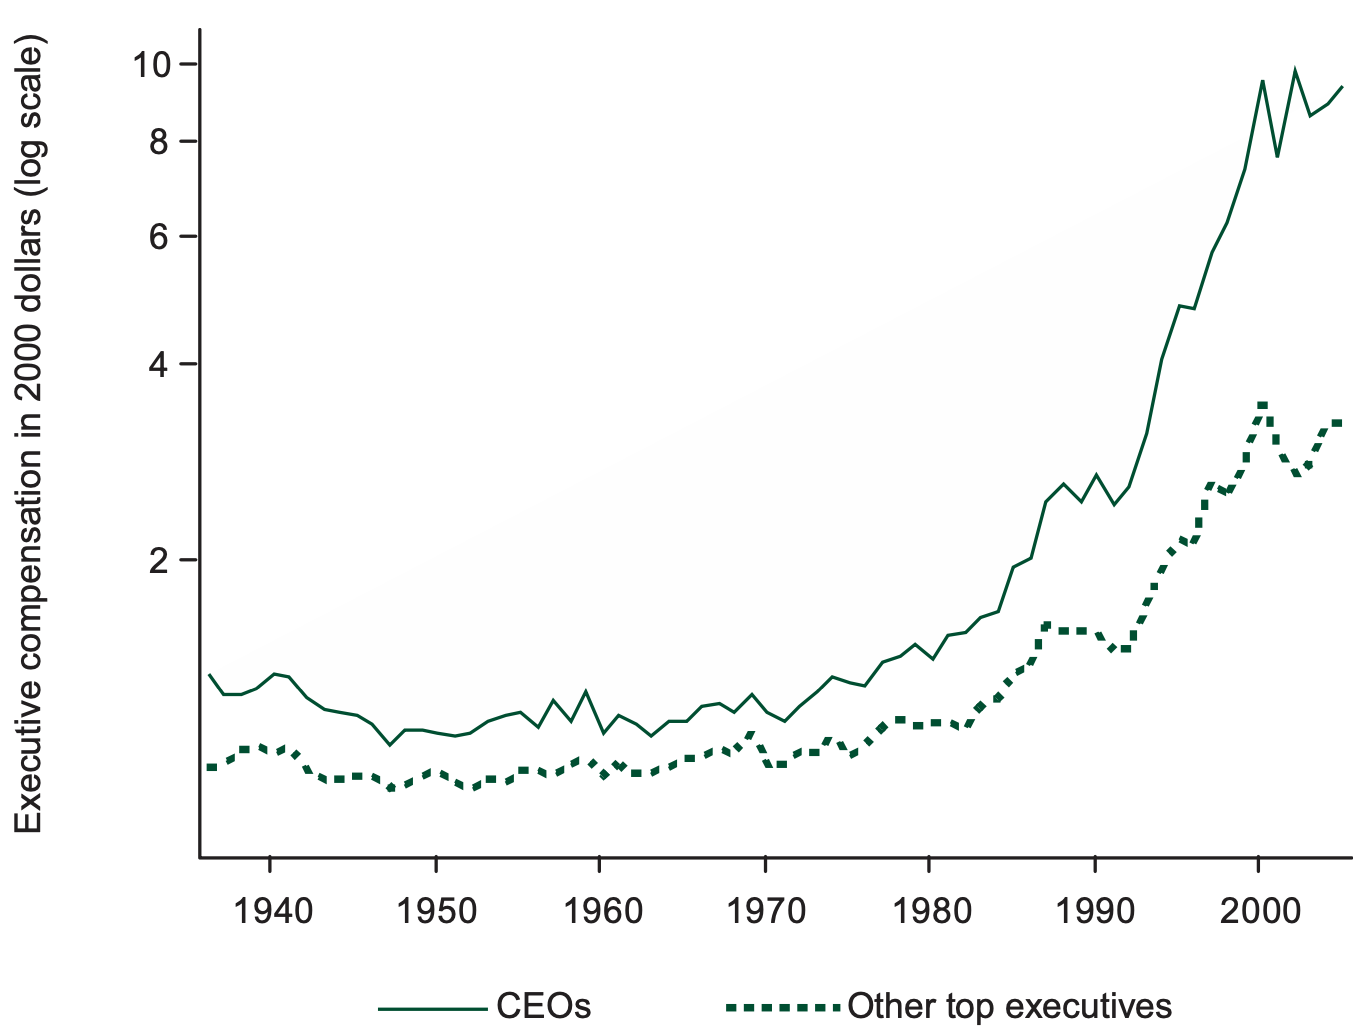
\includegraphics[width=0.6\textwidth]{fig/2/Frydman_fig1.png}
    \caption{Median compensation of CEOs and other top officers, 1936-2005 (Fig. 1 in \cite{frydman2010ceo})}
    \label{fig:frydman_fig1}
\end{figure}
\vspace*{15pt}


The reasons about the regime change are still debated. On one hand, we have the competitive hypothesis, which argues that the rise in CEO pay is the result of competitive forces, which have increased the demand for talented executives and thus their pay. On the other hand, we have the managerial power or rent extraction hypothesis, which argues that the rise in CEO pay is the result of powerful managers setting their own compensation. Both the exogenous and the endogenous hypotheses are consistent with empirical evidence, but neither is sufficient to explain the rise in CEO pay on its own \cite{frydman2010ceo}. \cite{edmans2017executive} highlights the importance of institutional forces, such as legislation, taxation, accounting policies and accounting standards; the latter were already emphasized by \cite{hall2003trouble} as a key driver of the rise in ESOs in the 1990s. 


Nevertheless, the last years have marked a modest trend-reversal in the use of ESOs. \cite{frydman2010ceo} shows that stock options made almost half of the total compensation package at the end of last century, with the percentage decreasing to 25\%-30\% in the 2010s, in favor of other means of performance-based compensation. See also figure \ref{fig:leung_tab_1-1} for the evolution in the number of firms in S\&P500 granting options and their average vesting period and time to maturity. The answer to whether stock or options are better means of compensation remains still open: as an example, \cite{kadan2008stocks} argues that stocks are preferable only when the nonviability (bankruptcy) risk is high, otherwise options are preferable for incentive purposes. 
More recently, the debate has however focused on the increasingly high levels of CEO pay, especially in the US, where by 2014 the median CEO in the S\&P 500 earned \$10.1 million per year, a sixfold increase from 1980 \cite{edmans2017executive}, contributing to a rising economic inequality \cite{mishel2012ceo}.

\vspace*{15pt}
\begin{figure}[H]
    \centering
    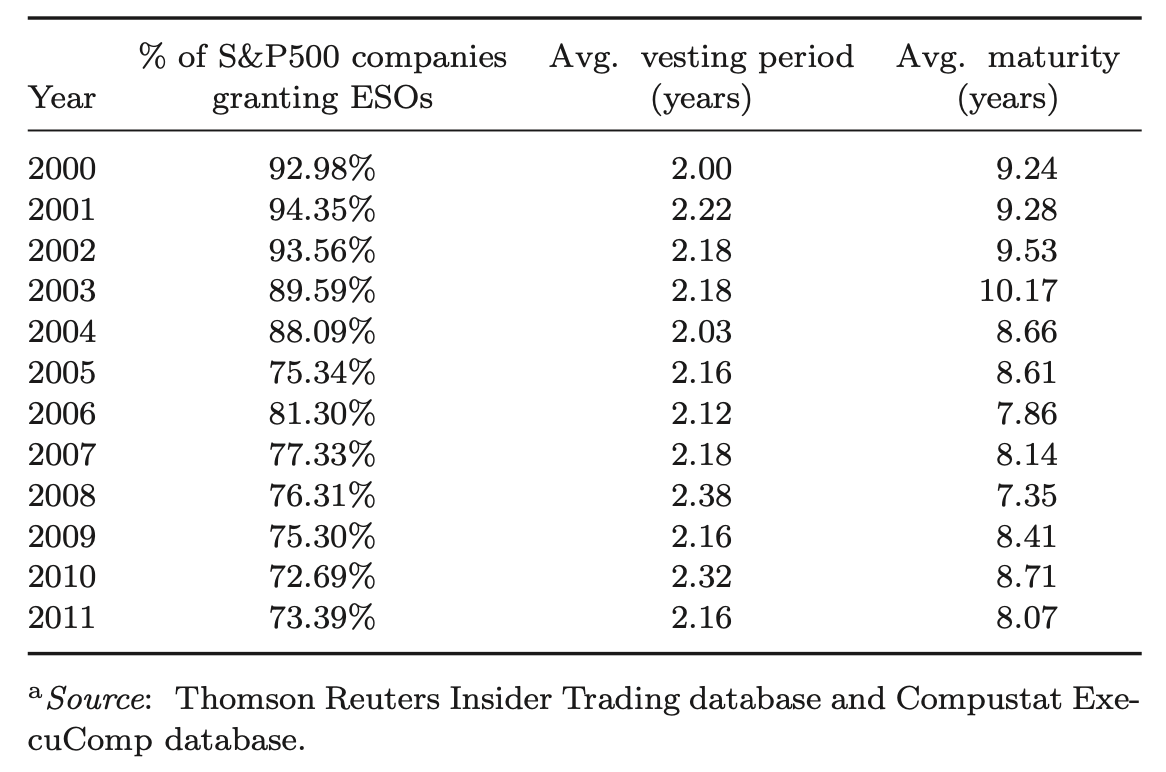
\includegraphics[width=0.6\textwidth]{fig/2/Leung_tab1-1.png}
    \caption{Summary of ESO compensations, 2000-2011 (Table 1.1 in \cite{leung2021employee})}
    \label{fig:leung_tab_1-1}
\end{figure}
\vspace*{15pt}


\subsubsection{Incentive alignment} 
    The main reason for the adoption of ESOs is to align the incentives of the executive with those of the shareholders. The misalignment between the two started with the separation of corporate ownership and corporate control at the beginning of the past century, which led to the need for a direct link between executive's realized compensation and the firm's performance. Indeed, the shareholders capture most of the benefits while the employee bears most of the costs, and thus the need to link the employee's compensation to some performance measure, such as the stock price for publicly traded firms. 
    The sensitivity of executive wealth to the underlying stock price - delta, in the case of options - is seen as a measure of the incentive alignment between the executive and the shareholders. The higher the delta, the more the executive's wealth is tied to the stock price, and the more the executive will be incentivized to take actions that increase the stock price. However, \cite{coles2006managerial} argues this effect may not be linear, as the inclusion of more and more performance-based and equity-based compensation in the executive's pay package has led to a higher sensitivity of the executive's wealth to the stock price, which in turn has led to a higher risk-taking behavior by the executive. Indeed, there is strong empirical evidence of a causal relation between manager compensation and investment policy, debt policy, and firm risk. Higher sensitivity of executive wealth to stock volatility - vega, in the case of options - leads to taking riskier policies, and also when controlling for the delta it "implies significantly higher R\&D expenditures, less investment in property, plant, and equipment, and an increased focus" \cite{coles2006managerial}. However, the relation between vega and risk-taking may be less evident than it may appear \textit{prima facie} and be mainly a matter of accounting \cite{hayes2012stock}. A more recent study by \cite{billings2020can} suggest that risky policies, as measured by investment and return in R\&D, vary concavely instead of convexly with vega, meaning that the marginal returns diminish with increasing vega, and so incentives may not be aligned.
    Therefore, higher delta and vega seem to expose the executive to more risk - be it convexly or concavely - which may not be desirable from the executive's point of view after a certain point. This is especially true for risk-averse executives, who may prefer to have a more stable compensation package, even if it means sacrificing some upside potential. But not all risk is equal: some suggest that executives prefer systematic to idiosyncratic risk because it can be hedged against \cite{armstrong2012executive}, while others suggest that executives believe they can better predict or influence the resolution of idiosyncratic uncertainty \cite{heron2017stock}. This distinction of risks affects also the difference in valuation between cost of option and executive value \cite{meulbroek2001efficiency}.
    Therefore, striking a balance between risk and incentives is desirable both for the executive and the firm. For the firm, on one hand risk-averse executives are offered options so to undertake more risk than they would normally, which is desirable for them; but on the other hand, such as taking on too much risk to increase the value of the option, or taking on too little risk to preserve the value of the option \cite{grinblatt1989adverse}.

    Among the factors driving the adoption of ESOs, we find ownership concentration, liquidity, CEO and institutional ownership, investment intensity, historical market return \cite{pasternack2002factors}. Many argues also in favor of its convexity of payoff, which has been however strongly criticized by many. \cite{ross2004compensation} takes a strong standpoint arguing that no incentive scheme will make all agents more or less risk averse uniformly. He argues that it is not true assuming \textit{a priori} that a convex fee schedule will make an agent less risk averse and that a concave one will induce greater risk aversion: they are both necessary conditions, but each insufficient on its own. Therefore, we need to also consider whether the fee schedule moves the executive into the more or less risk averse domain of her utility function, and the possible marginal magnification effects which may result \cite{ross2004compensation}. \cite{hayes2012stock} also finds no strong evidence on the convexity of ESOs. 
    Nevertheless, it remains incomplete talking about incentives without considering the whole compensation package, which influences heavily the executive's risk taking behavior but also the value she puts on the options. \cite{carpenter1998exercise} was the first to provide a solid foundation for the difference between firm cost and the executive value for an ESO; a difference that was later confirmed also by \cite{meulbroek2001efficiency} and \cite{hall2003trouble}. In particular, \cite{meulbroek2001efficiency} argues that this difference originates in the difference to risk exposure between the two parties, since undiversified managers are exposed to total firm risk but rewarded only for the systematic portion of it. This would then lead to a higher cost of the option for the firm than the value of the same for the executive. Moreover, talking about the relevance of executive's wealth, she finds that "managers at the average NYSE firm who have their entire wealth invested in the firm value their options at 70\% of their market value, while undiversified managers at rapidly growing, entrepreneurially-based firms, such as Internet-based firms, value their option-based compensation at only 53\% of its cost to the firm" \cite{meulbroek2001efficiency}. This is consistent with the idea that the executive's wealth and risk aversion play a key role in the valuation of the ESOs. Along these lines, \cite{hall2002stock} presents the divergence between firm (opportunity) cost and executive value, arguing that the former is the value if the firm were to sell the tradable and hedgeable option to an outside investor, while the latter is the value for the executive, who is not able to hedge the option and is exposed to the total risk of the firm. These differences lead thus to a higher cost for the firm than the value for the executive.
    Finally, early exercise has been a widely studied topic in the literature. \cite{huddart1996employee} analyze early exercise behavior and show that early exercise is strongly related to recent stock price movements, the market-to-strike ratio, proximity to vesting dates, time to maturity, volatility, and the employee's level within the company. \cite{heron2017stock} and \cite{izhakian2017risk} also find that the volatility of the stock is inversely related to early exercise, and this seems to trace back to the executive's valuation of the ESO. On the contrary, \cite{grasselli2009risk} argue that utility-based ESO models do not predict early exercise, but rather market frictions (e.g., costly exercise) or liquidity needs (for this, see also \cite{murphy2019employees}) may be better predictors of early exercise. They suggest that these findings could imply that utility-based models assuming block exercise result in an underestimate of the value of ESOs. 
    We now turn to a short historical overview of the evolution of valuation practices of ESOs, which has been another quite debated topic. 

\subsubsection{Valuation issues}
    Valuation of ESOs has been a controversial topic already starting from the 90s. At first, companies were required to disclose them in the annual statements, but they were not obliged to expense them. This changed slightly in 1995, when the Financial Accounting Standards Board (FASB) published the FASB123 (\cite{fasb123}), which encouraged companies to adopt a fair-value-based method of accounting for stock options instead of the intrinsic-value-based method, without however making this mandatory. Indeed, most companies continued using the intrinsic-value-based method, which was less costly \cite{hull2004value}. 
    Moreover, Appendix B of FASB123 proposed a three-step valuation method for the fair valuation: (i) estimate the expected life of the ESO, (ii) use Black-Scholes or CRR binomial method to estimate the value, (iii) adjust ex-post to account for possibility of the employee leaving the company when vested. Therefore, two key parameters drive the valuation: the estimated expected life of the option and the employee exit rate during the vesting period. The proposed methodology has been heavily criticized, most notably by \cite{hull2004value} as they argued it fails to account some key distinctive elements of ESOs, such as the vesting period and the restrictions usually entailed with the grant of these options. They thus proposed an ``Enhanced FASB123'' model, which accounts also for the possibility of the employees leaving the company after the vesting period - and hence, exercising only if the option is in-the-money when leaving - and incorporates the employee's early exercise policy as a multiple of the strike price, so that when the current stock price is above such threshold the employee will exercise. 
    This, along with other critics, spurred an important revision of the standard in 2004, by which it "eliminates the alternative to use Opinion 25’s intrinsic value method of accounting that was provided in Statement 123 as originally issued. Under Opinion 25, issuing stock options to employees generally resulted in recognition of no compensation cost. This Statement requires entities to recognize the cost of employee services received in exchange for awards of equity instruments based on the grant-date fair value of those awards (with limited exceptions)" (\cite{fasb123_revised}).
    The controversy around the valuation of ESOs has been also fueled by the fact that the Black-Scholes-Merton model, which is the most widely used model for valuing ESOs, has been criticized for overstating both the executive value and the cost of the option (\cite{carpenter1998exercise}, \cite{meulbroek2001efficiency}, \cite{hall2003trouble}, \cite{ingersoll2006subjective}, \cite{carpenter2010optimal} \cite{frydman2010ceo}), due to some of its underlying assumptions not applicable to ESOs. A different approach has been to model the exercise decision of the executive as part of a more comprehensive maximization problem of the executive, taking into account also other decision-relevant features, such as optimal portfolio allocation, optimal stopping time, exit from the firm, choices of consumption and effort, and other factors (e.g., \cite{huddart1996employee}, \cite{ingersoll2006subjective}, \cite{grasselli2009risk}, \cite{carpenter2010optimal}). A different stream has tried to combine theory and data to estimate option values (see \cite{carpenter1998exercise}) to calibrate the model.

\subsubsection{Basic terminology}
    Before delving into further topics, we provide a very short terminology used in option pricing; some of these terms have already been mentioned throughout the previous pages.
    A call option is a financial instrument known as a derivative that conveys to the purchaser (the holder) the right, but not the obligation, to buy a set quantity or dollar value of a particular asset at a fixed price by a set date (maturity). Employee Stock Options are thus non-transferable long-term call options on the stock of their employer. It is clear that such call option appreciates when the stock price goes up, and loses (intrinsic) value when the stock price goes below the initial strike price. The opposite is true for put options, which give the right to sell the asset at a fixed price by a set date, which thus appreciate when the stock price goes down.
    ESOs are American options, since they can be exercised also before maturity. On the other hand, we have European options, that can be exercised only at maturity. We say that an option is in-the-money when the stock price is above the strike price, out-of-money when the stock price is below the strike price, and at-the-money when the stock price is equal to the strike price. Most ESOs are usually granted at-the-money or slightly out-of-money. 
    The difference between the stock price and the strike price is called the intrinsic value of the option, while the difference between the option price and the intrinsic value is called the time value of the option. The time value is thus the value of the optionality of the option, i.e., the value that accounts for the possibility of further appreciation of the option. If the option is granted at-the-money, at the grant date its value will be entirely time value (since the intrinsic value equals zero when the option is at-the-value); at expiry, the value is entirely intrinsic value, as there is no more time value left.
    As stated before, ESOs are a special type of American call options, since they come with some restrictions, such as non-transferability and restrictions on short-selling the underlying stock. Non-transferability means that the holder cannot sell the option to somebody else, as would usually do with traditional options. Restrictions on short-selling of the stock imply that the holder cannot (fully) hedge against the firm-specific risk of the option. Moreover, ESOs are usually granted with a vesting period, which is the time the employee has to wait before being able to exercise the option. Therefore, she can exercise from when the option has been vested up to the maturity date. We show a visual example in figure \ref{fig:rep_vesting}. 

    \vspace*{15pt}

\begin{figure}[!h]
\centering
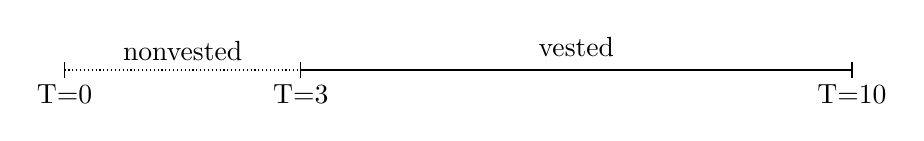
\begin{tikzpicture}
    % Draw horizontal line
    %\draw (0,0) -- (10,0);
    
    % Draw ticks
    \draw (0,-0.1) -- (0,0.1) node[anchor=south] {};
    \draw (3,-0.1) -- (3,0.1) node[anchor=south] {};
    \draw (10,-0.1) -- (10,0.1) node[anchor=south] {};
    
    % Add labels
    \node at (0,-0.3) {T=0};
    \node at (3,-0.3) {T=3};
    \node at (10,-0.3) {T=10};
    
    % Draw colored lines and labels
    \draw[densely dotted] (0,0) -- node[above] {nonvested} (3,0);
    \draw (3,0) -- node[above, yshift=1.5pt] {vested} (10,0);
\end{tikzpicture}
\caption{Visual representation of an ESO with 3y vesting period and 10y time to maturity.} 
\label{fig:rep_vesting}
\end{figure}

\vspace*{15pt}

    The vesting period is usually fixed, but may otherwise depend on some performance metric or the IPO of the company. Or, not all the options may be vested at once (cliff vesting), but options may be vested steadily in a uniform or non-uniform progression (graded vesting).
    Finally, we have the Greeks, which are the sensitivities of the option price to different factors.
    The delta of an option is the sensitivity of the option price to the stock price, while the vega is the sensitivity of the option price to the volatility of the stock. The gamma is the sensitivity of the delta to the stock price, while the theta is the sensitivity of the option price to the time to maturity. The rho is the sensitivity of the option price to the interest rate. The delta is usually positive for call options and negative for put options, while the vega is always positive. The gamma is always positive, while the theta is always negative. The rho is usually positive for call options and negative for put options.


\subsection{Reload options} %RED
    In its standard formulation, a reload option (also called restoration or replacement option) is a call option that, at exercise, grants a new option for every share tendered to exercise the original option. Therefore, if the holder exercises the option between expiry using previously owned company shares, she will receive, in addition to one share for each option exercised, a new option. Each new option has strike price set to the market price at time of exercise - so it is granted at-the-money - and the same maturity as the original option. We will consider them in the case of ESOs, so that both the original reload option and the new option granted at exercise are non-transferable and non-hedgeable.    

\subsubsection{Reload feature}
    Reload options were first developed in 1987 by Frederic W. Cook and Company for the Norwest Corporation, and they rapidly gained traction: 14\% of new stock option plans in 1996 and 17\% in 1997 were including them (\cite{dybvig2003employee}).
    The reload provision is nothing more than an option enhancement, whereby the exercise automatically triggers the award of new at-the-money options. This is indeed where the idea of recouping some time value comes into play: the holder exercises the option, receives the stock, and receives a new option at-the-money, which allows her to recover some time value sacrificed when exercising early the original option. Indeed, receiving an additional option allows to lock in a portion of the gain which could be possible, and of which time value is a manifestation. Another advantage is that the exercise does not change the manager's total equity holding but only its composition, which ties the executive to the firm's longer-term performance and is thus a desirable feature from an incentive perspective. Moreover, it encourages stock ownership, which is needed to enjoy the benefits of the reload provision at exercise. 
    \cite{hemmer2000reload} find that the optimal exercise policy is to exercise whenever the option as soon as it is in-the-money, which holds also when the option features a vesting period, a result confirmed later also by \cite{dybvig2003employee}. Reload options encourage early exercise as this allows to lock in a portion of the gain while retaining the same upside potential of the options \cite{hemmer1998optimal}. This is why the value of an option with a reload option is strictly greater than the value of the option without. But the same reason has been criticized for being a possible instrument of wealth transfer from the shareholders to the executives, a view that has been however criticized by \cite{dybvig2003employee} as not being supported by empirical evidence.
    Numerous modifications of the original reload option have been proposed and implemented in the stock option plans of many companies. For example, \cite{belanger2008infinite} studies a setting in which the reload option may be granted at a strike price higher than the stock price at exercise by a small percentage, and finds that both the exercise policy and the option value are very sensitive to small changes in this percentage increase. Similarly, \cite{dybvig2003employee} studies the case of an infinite reload option, which is a reload option that grants a new option at exercise for every share tendered, and finds that the value of the reload option lies between the value of the American option and the stock price, notwithstanding the number of reloads or the (possibly infinitely lived) time horizon of the option. Indeed, a holder could follow the American call's optimal exercise strategy and never exercise the reload option, which would make the value of the reload option equal to the American option. On the other hand, the stock price is an upper bound for the value of the reload option, as the holder could exercise the option and receive the stock directly. In particular, the value of the option is strictly smaller than the stock price when the stock grants dividends, as the dividends would not be enjoyed by the reload option holder. We now turn to a different modification of reload options, the so-called Dynamic Employee Stock Options.

\subsubsection{Dynamic Employee Stock Options}
    Dynamic Employee Stock Options (DESOs) were first proposed by \cite{huang2013dynamic} in 2013.  The difference with the traditional reload options is that the holder has more flexibility in the choice of the composition of the new options granted at exercise: for example, she can choose to receive 100\% stock (i.e., a traditional ESO), or to receive less than 100\% in stock but also some positive amount of ESO or restricted stock. The rationale behind the latter choice is that, similarly to the traditional reload options, this choice allows her to recover some time value at early exercise. They argue that this type of option has many advantages, both for the executive and the firm. The former avoids forfeiture of all time value when exercising early, reduces her overall risk at exercise by locking part of the gain, reducing thus the need for hedging. The latter enjoys cash flows from tax credits and tax deductions flowing in sooner, the executive is incentivized to take riskier projects sooner due to reduced overall delta risk, and allows attracting better talent due to an overall better compensation scheme. 
    They run a simulation with a 10-year DESO with a 3-year vesting period and a 10-year time to maturity, granting 75\% in stocks and 25\% in new ESOs at exercise and compare it with a traditional ESO. They find that such DESO costs only 4\% more than a traditional ESO, while providing the benefits to both parties. Therefore, the firm has a limited higher accounting cost while providing a better compensation scheme for the executive and a better alignment with the shareholders' interests. However, they do not elaborate on the subjective values of the two options to the executive.

\subsubsection{Valuation issues}
    Valuation is difficult due to the inherent heterogeneity in structuring the reload provision of the option. \cite{fasb123} states that the optimal valuation would be to consider the reload option when the option is granted at its fair value, but that no valuation method seemed able to do so. Therefore, "the Board concluded that the best way to account for an option with a reload feature is to treat both the initial grant and each subsequent grant of a reload option separately" \cite{fasb123}. However, this methodology was later shown to overstate the cost of the option (\cite{ingersoll2006valuing}). \cite{saly1999valuing} shows that it is possible to properly account for the reload feature using a binomial option pricing model, confirmed also by \cite{hemmer2000reload}. The latter showed also that the exercise policy is to exercise whenever the option is in-the-money, independently of the degree of risk aversion of the agent. However, \cite{saly1998ignoring} highlights that this is true for infinite reload options, but may not be true when the number of reloads is finite. Later, \cite{dai2005valuing} proposes a model which also accounts for the time vesting requirement.
    \cite{lau2005valuation} shows that also for reload options the values obtained via classical valuation and utility-based approaches show important differences. What is more, \cite{ingersoll2006valuing} finds that the deltas obtained via the utility-maximizing approach - the so-called subjective deltas - appear to be lower than the deltas obtained via binomial pricing - the so-called objective deltas - at least for infinite reload options. Finally, \cite{zhang2010knightian} propose a valuation model that is able to account also for Knightian uncertainty. As expected, they find that the value of the reload option to the Knightian-averse executive is lower as the coefficient of Knightian uncertainty increases.

    


\subsection{(Executive's) Risk aversion} %ORANGE
    Risk aversion is one of the fundamental ingredients in the rationale of ESOs. As we have seen, it motivates ESOs as incentive alignment mechanisms for shareholders that want to induce their risk-averse executives to take more risk. ESOs encourage risk taking, which compensates thus for the risk aversion of the executive. Therefore, it is expected that with ESOs, executives will take more risk than they would otherwise, which is desirable for the firm (up to some degree of risk taking, beyond which it could be detrimental). However, risk aversion also plays an important role in the valuation of ESOs, as the executive's risk aversion affects the value she puts on the options, which may differ from the cost of the options for the firm.
    Risk aversion is understood as the tendency for people to avoid or dislike risk. More formally, a preference $\succsim$ on a space of lotteries $\mathbb{L}$ over some consequences $\mathbf{C}$ is called risk averse if, for each lottery $l \in \mathbf{L}$, it holds $\EX[l] \succsim l$. This means that the expected value of the lottery is preferred to the lottery itself. A risk-neutral agent would have $\EX[l] \sim l$, while a risk-loving agent would have $\EX[l] \precsim l$. In the case of a vN-M preference, the preference allows for a utility representation $u$, whose concavity operationalizes the risk aversion: if $u$ is concave, then the agent is risk averse; if $u$ is linear, then the agent is risk-neutral; if $u$ is convex, then the agent is risk-loving. This allows also to rank risk aversions, as greater risk aversion is associated with greater concavity of the utility function, so that the utility function of a more risk-averse agent will be more concave than that of a less risk-averse agent, and in particular a strictly increasing transformation of the latter's utility function. Nevertheless, maybe the most famous characterization of risk aversion is by means of Jensen's inequality, stating that for a risk-averse agent it holds that $\EX[u(X)] \leq u(\EX[X])$ for some random variable $X$.
    Risk aversion affects block (\cite{grasselli2009risk}) and early exercise of options (\cite{izhakian2017risk}, \cite{murphy2019employees}): the exercise policy of American options prescribes indeed that a risk-neutral agent would not exercise earlier, if not for receiving some additional benefits of possessing the stock (e.g., dividends, voting rights, etc.). However, non-diversification and (more recently) liquidity constraints may lead risk-averse agents to exercise earlier, even though the two effects are unclear. \cite{carpenter2010optimal} argues that wealthier or less risk-averse executives exercise later and create greater option cost, while \cite{murphy2019employees} uses an exogenous appreciation of executive's home prices as proxy for increased wealth, showing that in this circumstance early exercise is driven by liquidity concerns rather than diversification purposes: in-the-money vested ESOs options provide thus easy access to cash to make major purchases. The liquidity hypothesis stands ground also because of implausibly high levels of risk aversion needed to justify early exercise and block exercise. 
    \cite{izhakian2017risk} consider also the role of ambiguity or Knightian uncertainty and finds opposing effects of risk and ambiguity on the incentive of early exercise of vested options: risk - measured in terms of equity volatility - causes executives to hold the option to preserve its time value (consistently with \cite{heron2017stock}), while ambiguity - defined as attitude towards mean-preserving spreads in probabilities - is positively related to early exercise. For the former, convexity of option payoff dominates concavity of utility function. The consideration of the role of ambiguity may be a promising venue for future research, as it may provide a more comprehensive understanding of the executive's behavior in exercising options and how it intertwines with risk aversion.
    Clearly, risk aversion coefficients of executives cannot be observed, but some studies have tried to estimate them from representative data on observable behavior. \cite{brenner2015risk} finds that heterogeneity in risk aversion coefficients among senior managers of boards of directors and non-senior executives, and that it is strongly correlated  with sector membership and firm-level variables such as size, performance, and capital structure. On gender differences, \cite{carter2017executive} finds that female executives hold significantly lower equity incentives and demand larger salary premiums for bearing a given level of compensation risk, suggesting thus higher risk aversion. But \cite{iqbal2006female} find that male executives engage in higher diversification-related stock sales than the female executives. Nevertheless, the literature on this remains scarce and more research is needed.

\subsection{Continuous principal-agent problems} %YELLOW
    Principal-agent problems have long been one of the most studied topics in the economic literature. The principal-agent problem arises when one party (the principal) delegates some decision-making authority to another party (the agent), who may have more information about the decision to be made. The agent's incentives may not be aligned with the principal's, and the principal may not be able to observe the agent's actions or characteristics. The principal's problem is then to design a contract that aligns the agent's incentives with her own, so that the agent will take the actions that are best for the principal. The agent's problem is to choose the actions that maximize her own utility, given the contract that the principal has offered. 
    The first models of principal-agent problems were static, one-period models, where the agent's action was observable by the principal. Future models incorporated the possibility of hidden actions or hidden characteristics, leading to the development of the moral hazard and adverse selection models. Adverse selection is usually modeled in terms of productivity or preferences, while moral hazard in terms of effort or risk choice (see \cite{cvitanic2017moral}). However, despite the simplifications that can be made on static models which render them a convenient tool, some features cannot be modeled well, such as firms' dynamics leading to cessation, private savings, and discounting. Dynamic setting allows also for modeling rewards over time, studying the variation of the level and sensitivity of pay, and employee exit dynamics \cite{edmans2017executive}. Therefore, dynamic models were developed to account for these features. The first dynamics models were treated as a series of one-period models, with continuous time being thus discretized in a series of time steps. A continuous-time generalization for the model in discrete time was first given by \cite{holmstrom1987aggregation}. They propose a model where the risk-averse and exponential utility agent controls the drift rate of some output process with built-in random fluctuations. They show that the optimal contract is linear in aggregate profits, which is consistent with the empirical evidence. The model has since then been extensively studied and extended in different directions: for example, \cite{schattler1993first} develop a first-order approach to the principal-agent model to an optimal stochastic control problem and relax the exponential utility requirement, while \cite{sung1995linearity} limit the model to CARA preferences but extend it by allowing the agent to control the diffusion-rate process, showing that the optimal contract remains linear.
    We will focus on the application of the relevant literature on dynamic models to the case of ESOs, but different approaches have been proposed (for example, \cite{plambeck2000performance} suggested using Markov decision processes). 
    The continuous-time approach has many advantages over the discrete-time one, among which ``tractability (which stems from the differential equation that characterizes the optimal contract), clarity (discrete-time models become messy very quickly), and computing power'' \cite{sannikov2013contracts}.  

    \cite{sannikov2008continuous} proposes a landmark infinite horizon model where payments are made continuously as function of past effort, rather than as a lump-sum payment at terminal date. The output is a diffusion process whose drift is determined by the agent's unobserved effort. The agent is risk-neutral, while the principal is risk-averse and enjoys consumption influenced by the agent's costly effort. The agent has the possibility of retirement. The model is solved by a system of coupled forward-backward stochastic differential equations, which are then solved numerically.
    The novelty of the paper is that the complete information case can be solved using the continuation variable as the only state variable; with moral hazard and adverse selection, the continuation value is not the only state variable anymore. \cite{sannikov2008continuous} solves for finite time horizon in this case, while \cite{cvitanic2013dynamics} solves for infinite time horizon where the agents are subject to an initial private shock. \cite{williams2009dynamic} proposed a more generic method, for which only a partial characterization is however possible. 
    Cvitanić has a good stream of papers of moral hazard and adverse selection in continuous time: for example, with some constant private shock that has a long-lasting effect \cite{cvitanic2013dynamics}, or a dynamic programming solution to a problem with lump sum payment by restriction of the set of feasible contracts and generalization of utility function (\cite{cvitanic2018dynamic}). With Cadenillas and Zapatero, he applies this dynamic setting to ESOs, whereby the agent can influence the stock by exerting costly effort and through the choice of projects that influence the volatility. In \cite{cadenillas2002executive} they solve for the firm's optimal strike price and compute it numerically for the logarithmic case, and in \cite{cadenillas2005executive} they argue that options may be an effective mechanism to screen out bad executives, as adverse selection requires more leverage than the perfect information case.
    Finally, the advent of computational power, as well as the need for solving analytically many backward stochastic differential equations, has led to a stream of research focusing on computational solutions when closed-form solutions are not feasible (\cite{azar2018computational}, \cite{dutting2021complexity}, \cite{dutting2023multi}). 




%Small concluding paragraph
Decades of research but still many open unanswered questions...




